% Introduction

% Main chapter title
\chapter{Partitioning of Tanner Graph} 

% Change X to a consecutive number; for referencing this chapter elsewhere, use \ref{ChapterX}
\label{Chapter6} 

% This is for the header on each page
\lhead{Chapter 5. \emph{Partitioning of Tanner Graph}}  

\section{Introduction}
The literature survey about hardware implementation of the LDPC decoder concludes three different implementation strategies.The serial decoder is the simplest decoder. Hardware cost and complexity is very less. It consists of single check node, single bit node and memory. The bits are first passed one by one from bit side to check side and generated checks are stored in memory, then checks are passed from check side to bit side one at a time to update the bit nodes. The main drawback is this implementation is too slow \cite{4}. The second approach is implementing a fully parallel algorithm. This is a direct implemention of the Tanner graph in hardware [5]. This increases the decoding speed, but hardware cost and implementation complexity becomes too high. Another approach is midway between serial and parallel, called partial parallel implementation. This implementation is more flexible as trade off between speed and cost can be done. In partial parallel implementation bit nodes and check nodes are divided into several partitions. All these partitions works in parallel, but within one partition the information is transferred serially. Larger the number of partitions, faster the decoder as it acts more like parallel decoder. Fewer the partitions, simpler the decoder as it acts more like serial implementation of the decoder. Thus, we can trade off between speed and cost. Further, a reconfigurable interconnection network has to be designed to change the connection from bit to check side for different iterations in partial parallel decoder. The multistage interconnection network provides cost efficient parallel processing. Non-blocking and rearrangable networks are preferred. In blocking network connection is not always possible, whereas non-blocking network always provides a path between input to output. A rearrangable network can always provide a path, but path has to be rearranged. Lee and Ryu have used Benes network in their partial parallel LDPC decoder \cite{5}. Benes network is a rearrangable network.

\section{Partitioning}
To use the partial parallel approach we propose to iteratively decompose the Tanner graph into sets of bits and sets of checks. In one iteration one set of bits is transferred towards one set of checks. It will be preferred that maximum number of the computational bits required for a particular check set are in same bit set so that computation can be completed for as many check nodes as possible. If a check set requires bits from many bit sets, then the number of iterations required to complete the computation of that set will be equal to the number of bit sets required to perform all the computation. Thus, if many check sets require bits from a large number of bit sets, then number of iterations increases and decoding time will become worse. Thus, an efficient partitioning of bit and check side of the Tanner graph is required. \\
The objective is to partition the bipartite graph corresponding to parity check matrix into two subsets in both bit side and check side such that most of the edges of a set of bit side relates to a particular set of check side. We call these edges as \lq Through edges\rq. The remaining edges of the same set on the bit side that goes to different set in check side are called \lq Transverse edges\rq. The average ratio of total number
of through edges to total number of edges is the performance index for parallelization. \\
Suppose we have bipartite graph G, bits are
B = \{ $b_{1}$ , $ b_{2}$ ,$b_{3}$ ,...,$b_{n}$ \} and checks are C=\{ $c_{1}$,$c_{2}$ ,$c_{3}$,...,$c_{m}$ \}
and the edge between bit node $b_{i}$ and check node $c_{j}$ is represented as $e{i,j}$. Now we have to partition G into four subsets $B_{1}$ ,$B_{2}$ ,$C_{1}$ and $C_{2}$ such that
\begin{itemize}
\item   Size of set$ B_{1}$ and set $B_{2}$ should be nearly equal as well
as size of$ C_{1}$ $and C_{2}$ should be nearly equal.
\item  There should be a very small number of edges between
$B_{1}$-$C_{2}$and $B_{2}$-$C_t{1}$so that the number of cross edges are minimised. 
\end{itemize}


 \begin{figure}[h]
 \begin{center}
    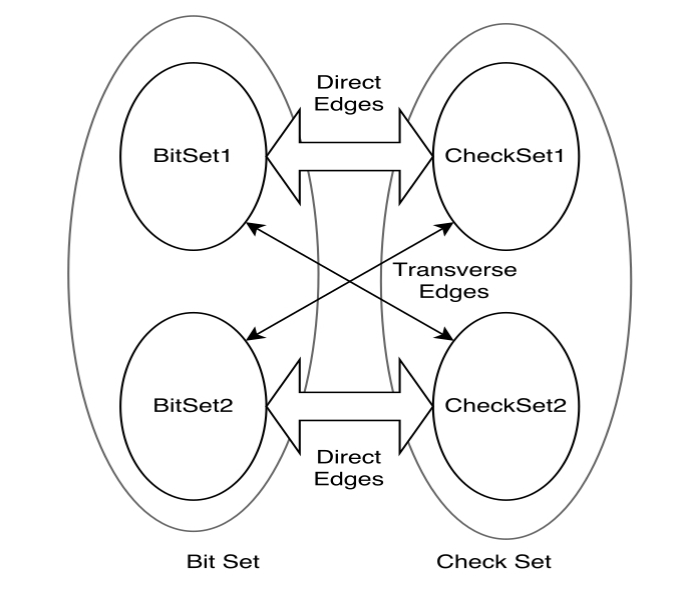
\includegraphics[height=8cm,width=8cm]{partition1.jpg}
    \caption{Partitioning a bipartite graph} 
 \end{center}
\end{figure}


\section{Procedure}
To approach this we initially find a weighted check matrix from the parity check matrix. The weighted check matrix is an incidence matrix for the check node graph. A check node graph is a weighted graph. The weight between $checknode_{i}$ and $checknode_{j}$ is the number of common bit nodes performing check on both $checknode_{i}$ and $checknode_{j}$ . After forming the
weighted check graph we partitioned it into two equal parts using METIS \cite{6}. After partitioning the check set into two equal sets with minimum weight cut, we need to partition the bit set. To partition the bit set we take into account the number of checks associated with a bit. If number of checks associated with a bit are more in first check set then it goes to first check set else it goes to second check set. As all matrices are sparse, the number of bits divided in two sets comes out nearly equal. To make them exactly equal we force some bits to go to other set after partitioning. Then the average ratio of parallelized edges to total edges and transverse edges to total edges is calculated as a performance index of parallelization of the
decoder. Figure \ref{partition2} shows the block diagram for the process of partitioning the bipartite graph corresponding to a low density parity check matrix.


 \begin{figure}[h]
 \begin{center}
    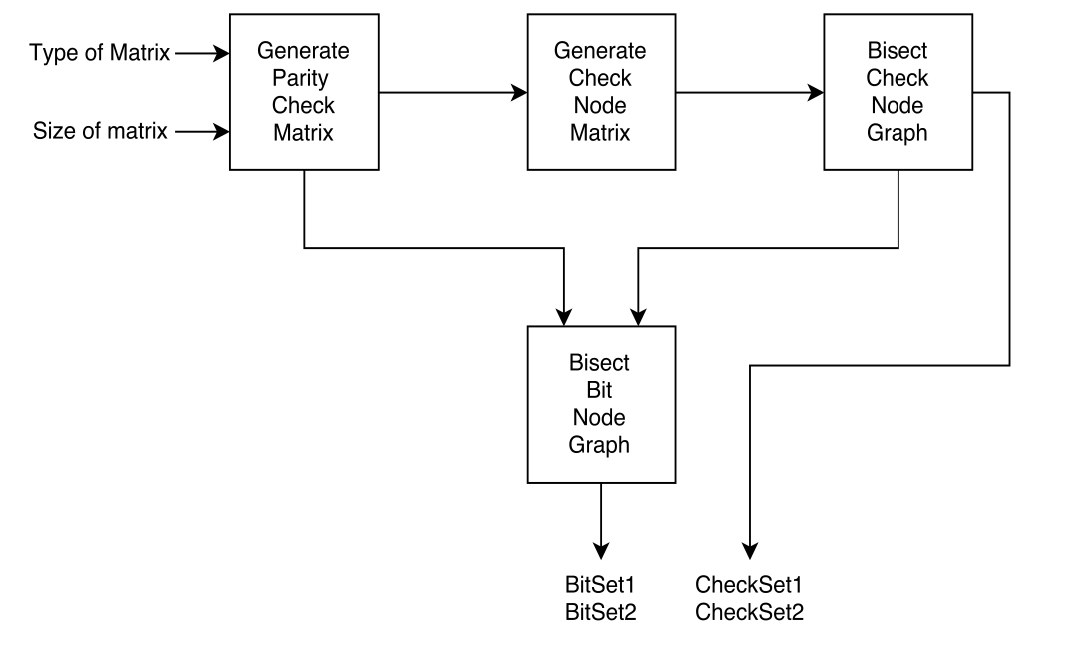
\includegraphics[height=8cm,width=14cm]{partition2.jpg}
    \caption{Block Diagram of process flow} 
    \label{partition2}
 \end{center}
\end{figure}  

\begin{itemize}
\item \textbf{Generation of Parity Check Matrix}
\item \textbf{Generation of Check Node Incident Matrix} \\
The weight between two check nodes is the number of common bit nodes performing exor operation on both check nodes.
Taking this into account, we followed following algorithm to
convert a parity check matrix to a check node incidence matrix.

\item \textbf{Bisection of Check Node Graph}

Partitioning of check node graph is done using METIS \cite{6}.
"METIS is a set of serial programs for partitioning graphs,
partitioning finite element meshes, and producing fill reducing
ordering for sparse matrices. The algorithms implemented in
METIS are based on the multilevel recursive-bisection, multilevel k-way, and multi-constraint partitioning schemes"\cite{6}.
First, the incidence matrix is converted into a corresponding
graph format that can be given as input to METIS. At output
we get two partitions of equal size with the minimum weight
cut.

\item \textbf{Bisection of Bit Node Graph}

After bisection of the check set we get two sets $C_{1}$ and $C_{2}$ .
Now, we have to divide a partition of bit set into $B_{1}$ and $B_{2}$ . A
bit node corresponds to set $ B_{1}$ if the number of edges between
that bit node and set $C_{1}$ are more than the number of edges
between bit node and set $ C_{2}$ . As the check set is bisected by
keeping in mind that the more the number of checks relating
to a bit are in same set and the matrix is sparse thus we get
nearly equal bits in set $B_{1}$ and set $B_{2}$. As this bisection has
to be further iterated for partitioning, we force the bisection
to be equal. Forcing the bisection to be equal increases the
transverse edges.


\end{itemize}

\section{Results of partitioning applied to matrices}
Simulation for partitioning are performed in MATLAB environment. Figure \ref{gallager_part} shows the performance index for Gallager matrix when we vary the order of the parity check matrix from 1,000 to 10,000. The performance index comes 0.78 for Gallager matrix. Similarly, by varying the order of the parity check matrix from 1,000 to 10,000 we get performance index of MacKay Neal matrix as 0.88, depicted in Figure \ref{makey_part}. Quasi Cyclic matrix can be formed only for a special set of numbers. In simulation, the order of matrix taken are 155, 305, 905 and 11555,
and performance index is above 0.88 in all cases, as depicted in Figure \ref{qc_part}.

 \begin{figure}[h]
 \begin{center}
    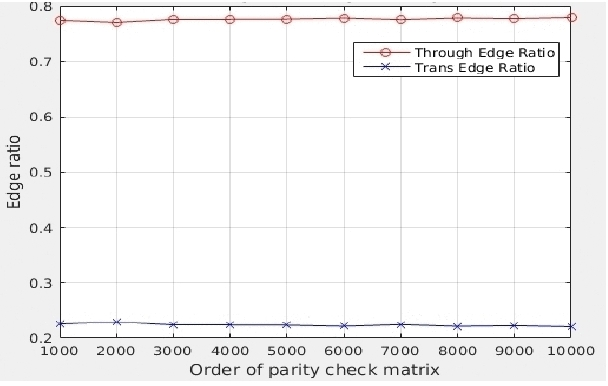
\includegraphics[height=8cm,width=12cm]{gallager_part.jpg}
    \caption{Performance of Gallager matrix}
    \label{gallager_part} 
 \end{center}
\end{figure}   
 
  \begin{figure}[h]
 \begin{center}
    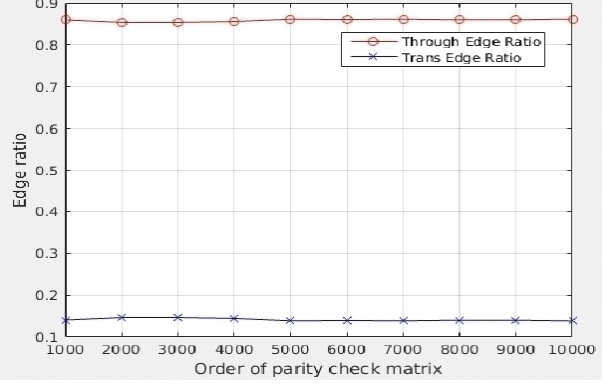
\includegraphics[height=8cm,width=12cm]{makey_part.jpg}
    \caption{Performance of MacKay Neal matrix} 
    \label{makey_part}
 \end{center}
\end{figure}


 \begin{figure}[h]
 \begin{center}
    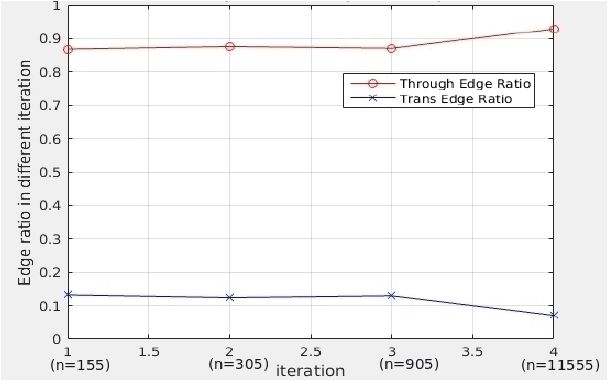
\includegraphics[height=8cm,width=12cm]{qc_part.jpg}
    \caption{Performance of quasi-cyclic matrix} 
    \label{qc_part}
 \end{center}
\end{figure}
